\section{Theorie}
\label{sec:Theorie}
\subsection{Allgemein}
Wirken Kräfte auf einen Körper, so kann die Form und das Volumen des Körpers verändert werden.
Die Kräfte beziehen sich meist auf die Flächeneinheit und werden als Spannung $\sigma$ bezeichnet.
Die senkrecht zur Oberfläche wirkende Spannung wird als Normalspannung bezeichnet.
Tangential- oder Schubspannung heißt hingegen die parallel zur Oberfläche verlaufende Komponente.
Liegt bei der relativen Längenänderung $\frac{\Delta L}{L}$ ein linearer Zusammenhang vor, so beschreibt das Hook'sche Gesetz
\begin{equation}
    \sigma = E \cdot \frac{\Delta L}{L}
\end{equation}
die Deformation.
Dabei beschreibt $E$ der Elastizitätsmodul, $L$ die Länge und $\Delta L$ die Längenänderung des Körpers (siehe Abb. \ref{fig:spannung}).
Der Elastizitätsmodul ist eine materialabhängige Konstante des Werkstoffes.
Die Längenänderung $\Delta L$ kann nur mit genauen Messaperaturen direkt bestimmt werden.\\
Eine weitere Möglichkeit zur Bestimmung des Elastizitätsmodul ist die Biegung.
Hier genügt eine relativ kleine Kraft am Ende des Stabes um eine messbare Längenänderung zu bewirken.
\begin{figure}
    \centering
    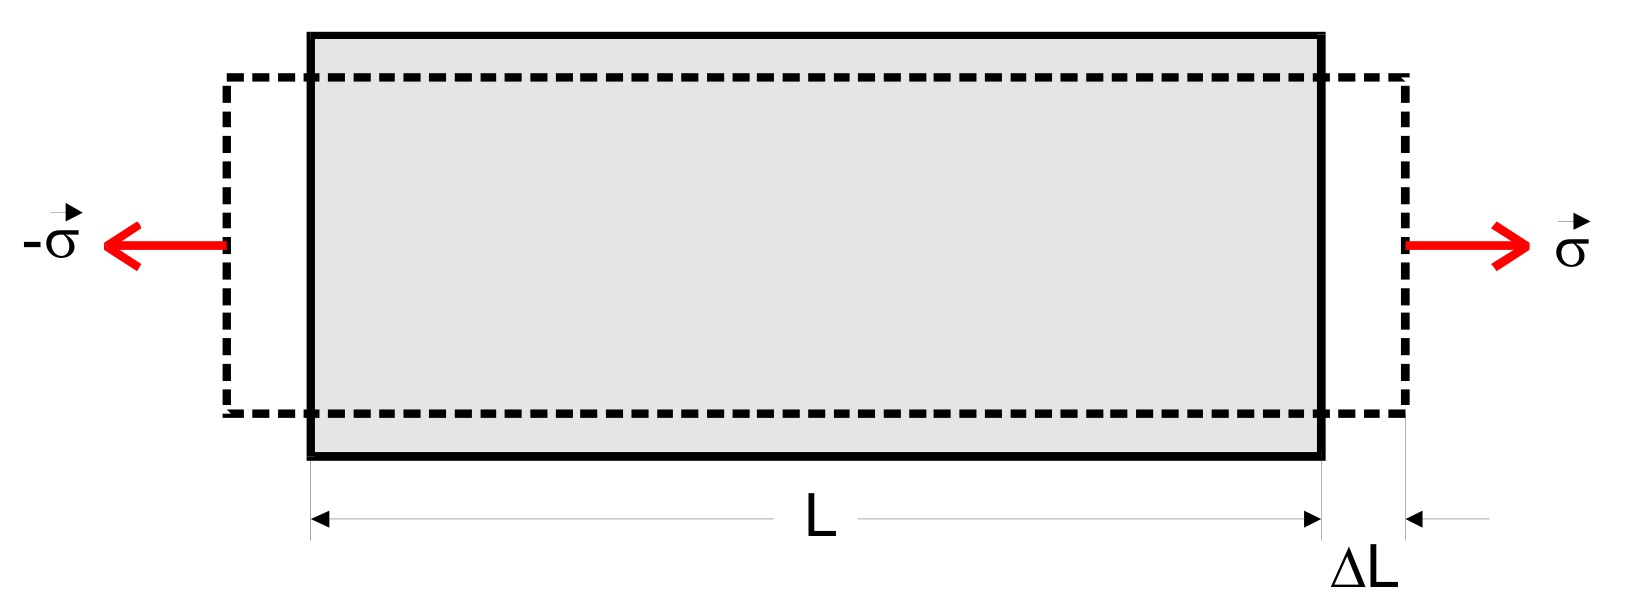
\includegraphics[width=0.75\textwidth]{content/data/spannung.jpg}
    \caption{Dehnung eines Stabes bei wirkender Normalspannung.\cite{anleitung}}
    \label{fig:spannung}
\end{figure}
\subsection{Biegung - einseitige Einspannung}